%----------------------------------------------------------------------------------------
%	OPACITY
%----------------------------------------------------------------------------------------
%\section{Opacity derivation}
%\label{se:opacities}
%
% LP: copie de l'intro de Xavier
In NIKA2, the opacity is measured via a total-power technique, which was successfully tested with NIKA. The details of this technique and its agreement with the Atmospheric Transmission at Microwaves (ATM) model (\cite{2001IEEE....49.1683C}) are described in \cite{Catalano2014}. The underlying idea is to replace the opacity, usually delivered by the resident IRAM tau-meter that performs elevation scans at a fixed azimuth and is operating at 225\,GHz, by a measurement that uses the NIKA2 instrument itself as a tau-meter. Using this procedure we can directly derive an opacity integrated in the NIKA2 very bandpasses and in the same line-of-sight of the source in the considered map. First, we have to calibrate the relationship between total power and opacity.
% fin copie

\subsection{Methodology}
For each kid $k$, the absolute value of the resonance frequency
$f_{tone}^k$ moves with the atmospheric load according to

\begin{equation}
f_{tone}^k = C_0^k + C_1^k T_{atm}[1-e^{-\tau/\sin\delta}]
\end{equation}

{\bf LP: pourquoi signe plus alors qu'on utilise un signe moins dans
  Eq. 2 du papier instru ?}

where $C_0^k$ is a constant equal to the resonance
frequency at zero opacity, $C_1^k$ is the calibration conversion
factor in kHz$/$K, $T_{atm}$ is the equivalent temperature
of the atmosphere (taken as a constant at 270K), $\tau$ the zenith
opacity and $\delta$ the average elevation of the telescope.
By assuming a homogeneous plane-parallel atmosphere, the airmass $x$ is defined from the
elevation as $x = \sin\delta$. 

The coefficients $C_0^k$ and $C_1^k$ are expected to be constant in time
within at least a cooldown cycle, and are determined using a {\tt
  skydip} procedure. This consists in moving
the telescope in elevation step by step and to monitor, for each kid, the
evolution of $f_{tone}^k$ vs the air mass and to fit the zenith opacity $\tau$ and
$C_0^k$ and $C_1^k$. Namely, during a {\tt skydip}, the telescope performs
eleven elevation steps in the elevation range from 19 to 65 degrees, regularly
spaced in airmass. For each step, we acquire about twenty seconds of
time traces to reduce the error in the determination of $f_{tone}^k$.

All the skydips (that were obtained under various opacity
conditions) are analysed together to break the degeneracies between
the opacity and the responsivity. The procedure has two steps.
First, all the skydips are analysed individually to simply measure
$f_{tone}^k$ for each stable elevation and fit simultaneously all the
parameters ($\tau$, $C_0^k$ and $C_1^k$.)
Error bars on $\tau$ are estimated by doing
this procedure on blocks of 40 kids only and getting a dispersion on the
resulting $\tau$ from the different blocks. Usually the dispersion comes out as
$4\times 10^{-3}$ at 1mm and $1\times 10^{-3}$ at 2mm. Once the $\tau$ values
are estimated for each skydip (as the average over the blocks), we compute
(while fixing $\tau$) the $C_0$ and $C_1$ final values for each KID. We thus
retrieve the coefficients of all the KIDs even though some of them could not
contribute to the tau determination.

%% \begin{figure}
%% \begin{center}
%% 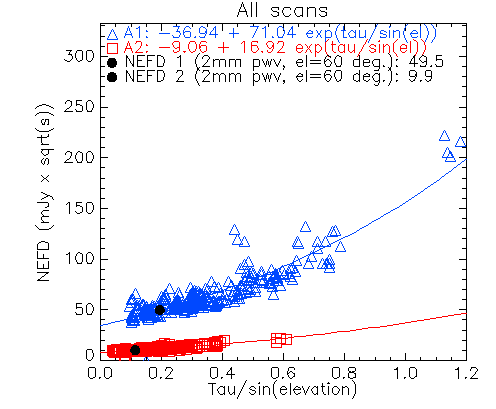
\includegraphics[clip, angle=0, scale =
%%   0.5]{Figures/NEFD_vs_tau_20170226s415_FXDC0C1_Jy_common_mode_kids_out.png}
%% 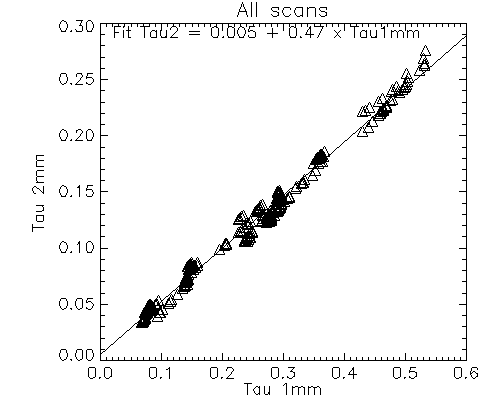
\includegraphics[clip, angle=0, scale =
%%   0.5]{Figures/tau1_tau2_20170226s415_FXDC0C1_GaussPhot_common_mode_kids_out.png}
%% \caption{}
%% \label{fig:fov}
%% \end{center}
%% \end{figure}

%  figure deplacee dans Opacity_checks.tex
%\begin{figure}
%\begin{center}
%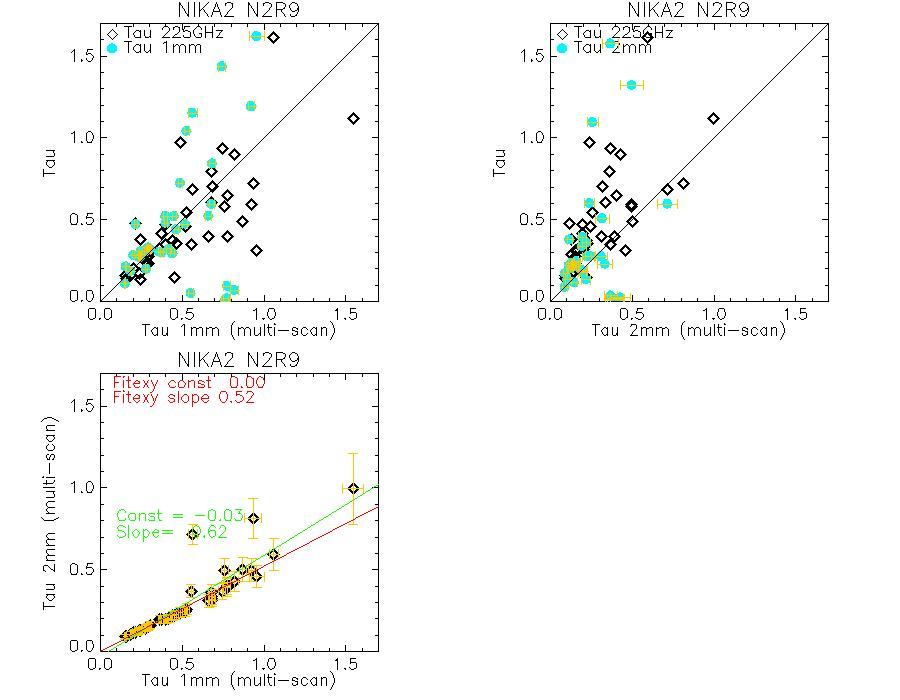
\includegraphics[clip, angle=0, scale = 0.5]{Figures/test_allskd_N2R9.jpg}
%\caption{{\bf Fix me : improve plot quality and plot only the 3rd one.}}
%\label{fig:test_allskd_N2R9}
%\end{center}
%\end{figure}

%\subsection{Opacity measurement consistency tests}

%{\bf copy from the 'Instru' paper}

\begin{figure}[ht]
\begin{center}
\includegraphics[scale=0.8]{Figures/test_allskd_N2R10v2commiss2.pdf}
\caption{Atmospheric opacity as measured from the NIKA2 data 
at 260 (top) and 150\,GHz (bottom) during N2R10
commissioning campaign. Each block of 40 KIDs gives an independent estimate of
the opacity value for each skydip scan (the integer abscissae). The block
number is the decimal value of the abscissae.
\label{fig:taumeas_paper}}
\end{center}
\end{figure}

\begin{figure}[ht]
\begin{center}
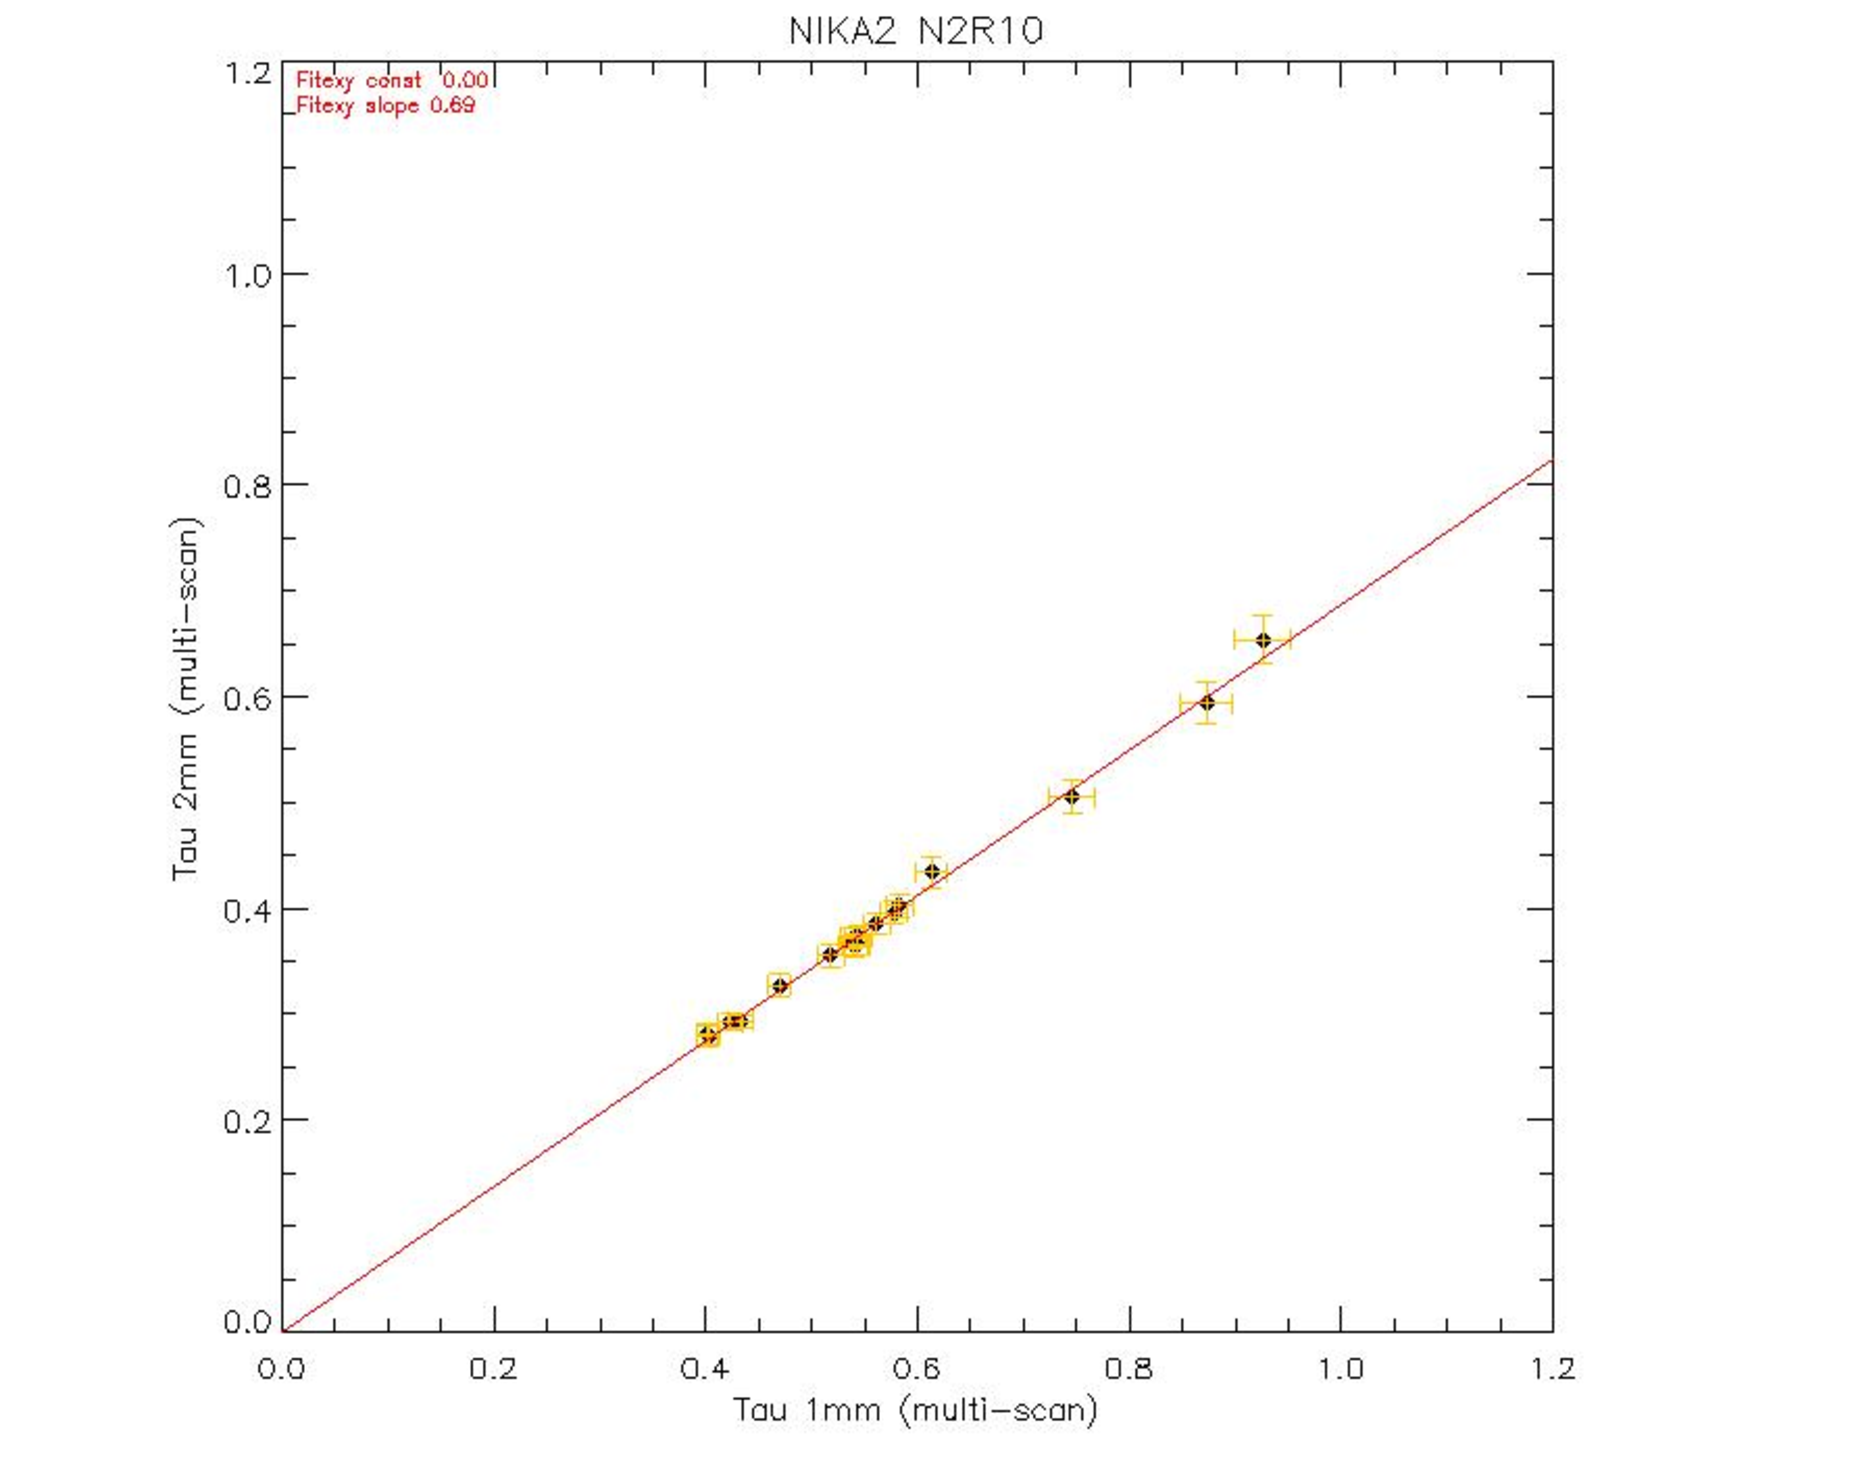
\includegraphics[scale=0.8]{Figures/test_allskd_N2R10v2commiss1.pdf}
\caption{Atmospheric opacity as measured from the NIKA2 data 
at 260 and 150\,GHz during N2R10
commissioning campaign. The error bars are in fact dispersion of the deduced
opacities between blocks of 40 KIDs.
\label{fig:taumeas_paper}}
\end{center}
\end{figure}

We observe that the skydip-fitted $\tau$ values are, as expected, common
between different detectors of the same array (the two 1mm arrays show
slightly different values). By comparing the results of different skydips, we
have verified experimentally that the coefficients $C_0$, $C_1$ are stable,
within the fit errors, on very long time scales within a cooldown cycle. The
coefficients can thus be applied to the whole observing campaign in order to
recover the opacity of each scan.


% \noindent {\bf FM : a figure would help to convince the reader that it is stable on lng time
% scale, which is a key point.}\\ FXD: I will do that figure


\begin{figure}[ht]
\begin{center}
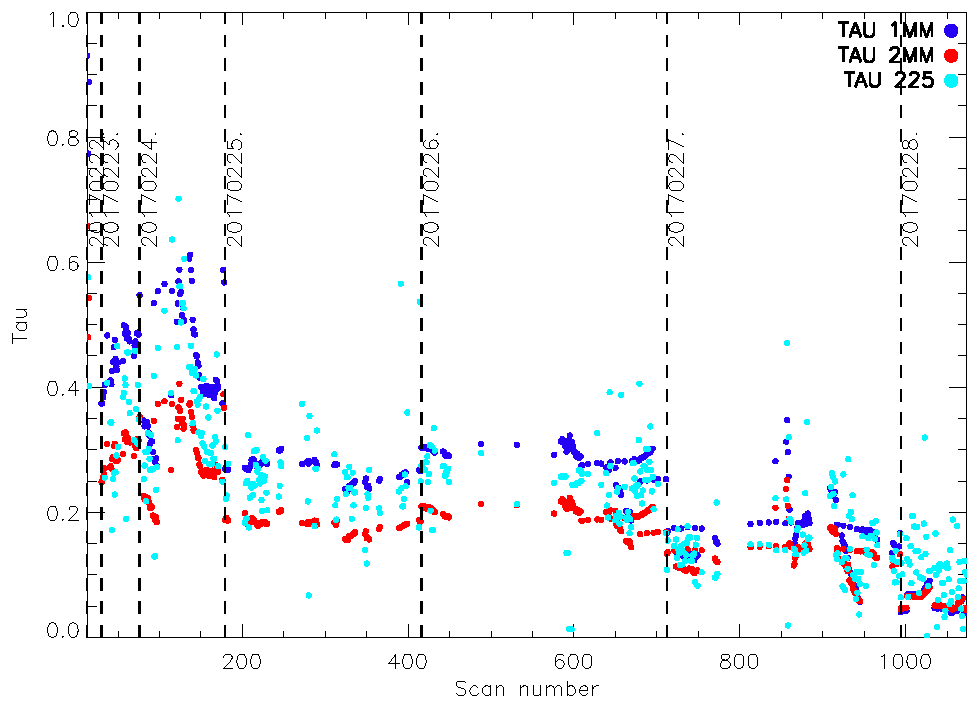
\includegraphics[scale=0.8]{../../Paper_NIKA2_Technical/opacity_evol_run22.pdf}
\caption{Atmospheric opacity as measured from the IRAM 225\,GHz taumeter
(cyan), and from the NIKA2 data at 150 (red) and 260\,GHz (blue) during N2R9
commissioning campaign (Feb. 2017). We stress the fact that the IRAM 225\,GHz
taumeter data is not used for the atmospheric correction and is plotted here
just for comparison.
  \label{fig:taumeas_paper}}
\end{center}
\end{figure}


\begin{figure}[ht]
\begin{center}
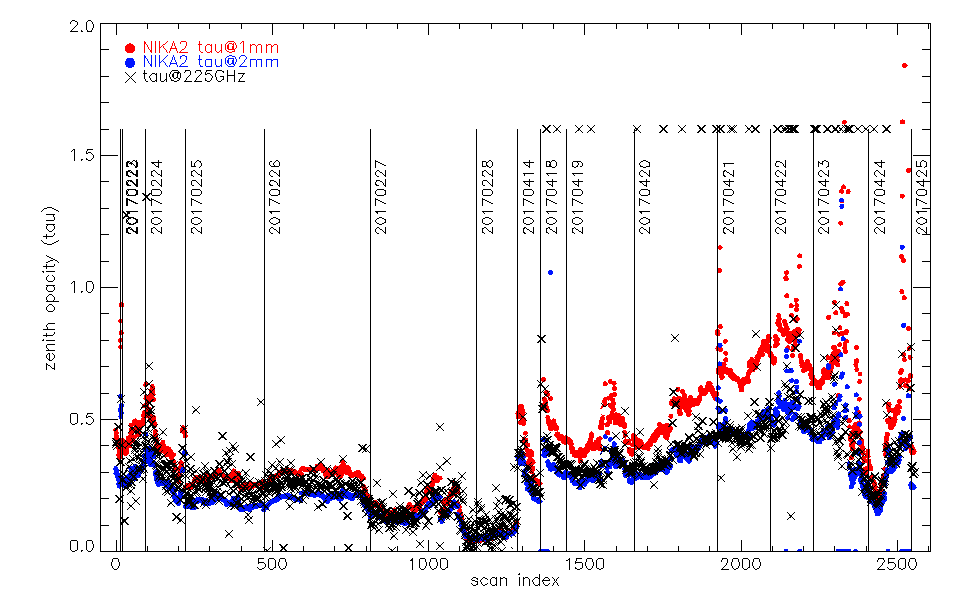
\includegraphics[width=\linewidth]{Figures/opacity_vs_index_N2R9_N2R10.png}
\caption{Atmospheric opacity as measured from the IRAM 225\,GHz
  taumeter (black crosses), and from the NIKA2 data at 150 (red) and 260\,GHz (blue) during 
  N2R9 and N2R10 commissioning campaigns.  We stress the fact that the IRAM 225\,GHz taumeter data is not used for the atmospheric correction and is plotted here just for comparison.
  \label{fig:taumeas}}
\end{center}
\end{figure}


In Fig.~\ref{fig:taumeas} {\bf(and Fig.~\ref{fig:taumeas_paper} of
  \ref{NIKA2-Tech}) } we present the evolution of the NIKA2 in-band
opacities for all the 'OTF' scans (about 1300 scans per runs) of the
N2R9 run held in February and the N2R10 run in April 2017. These are
compared to the IRAM tau-meter values. We observe an agreement on the global trend between the IRAM tau-meter opacity
(225 GHz) and the NIKA2 values. These latter show, however,
a smaller dispersion (less than one percent).
% {\bf FM : how small ?}.


We find an average ratio between the 150 GHz and the 260 GHz NIKA2 values of
about 0.6, a bit higher than ATM model expectations. We notice however that
the 150 GHz-to-260 GHz opacity ratio varies significantly for opacities (at
150 GHz) below 0.2. This effect is likely to be linked to an $O_2$ atmospheric
line which becomes saturated or to some spillover at 2mm. This point is,
however, still under investigation.''


% \noindent {\bf FM : a figure of the ratio of taus would be useful. It should be compared with  
% Fig. \ref{thopacities}, which should appear in this section ...}
% FXD: figure above gives the measured ratio. 


\begin{figure}[ht]
\begin{center}
  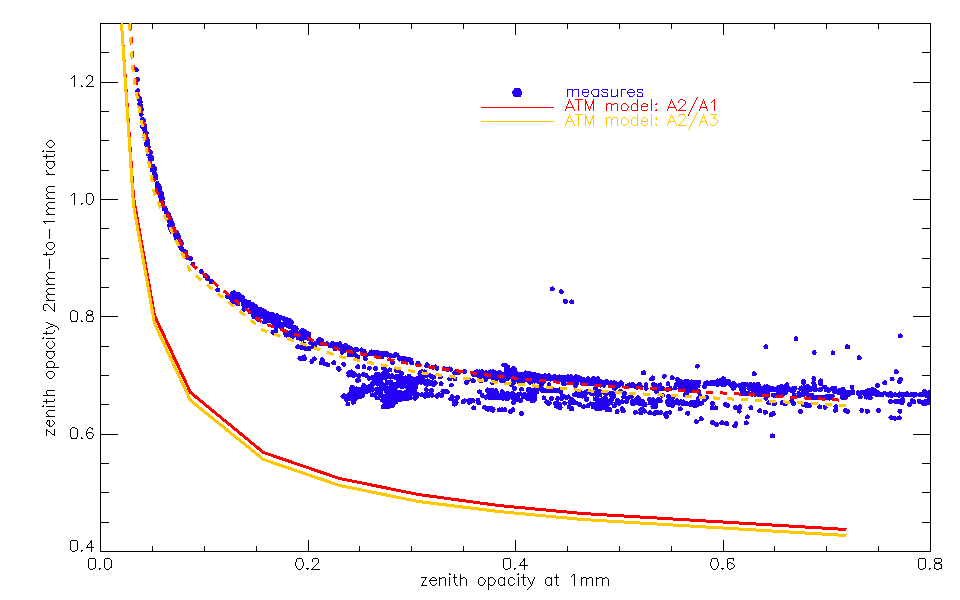
\includegraphics[width=0.65\textwidth]{Figures/opacity_tau1_tau2_ratio_N2R9_N2R10.png}
  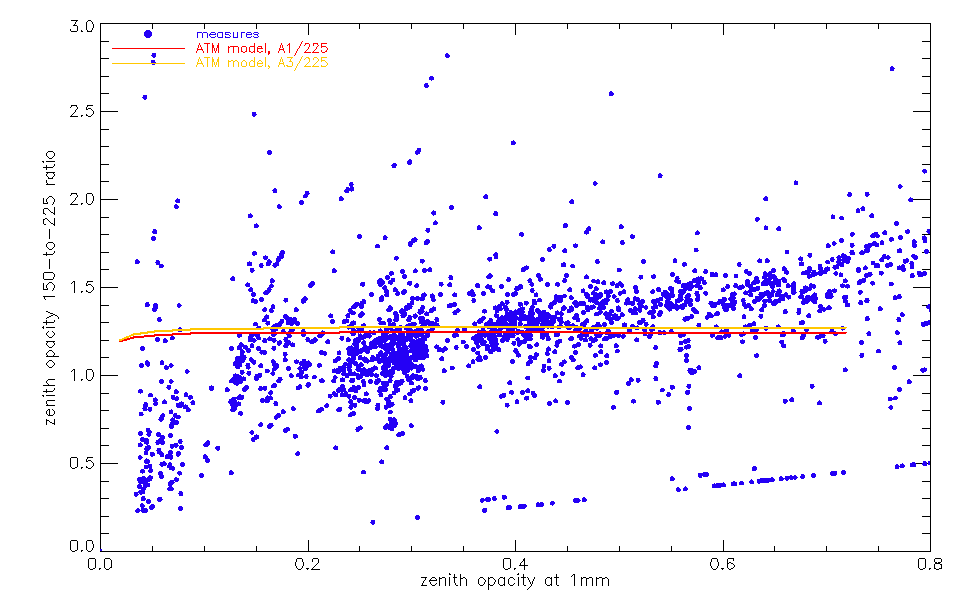
\includegraphics[width=0.65\textwidth]{Figures/opacity_tau1_tau225_ratio_N2R9_N2R10.png}
  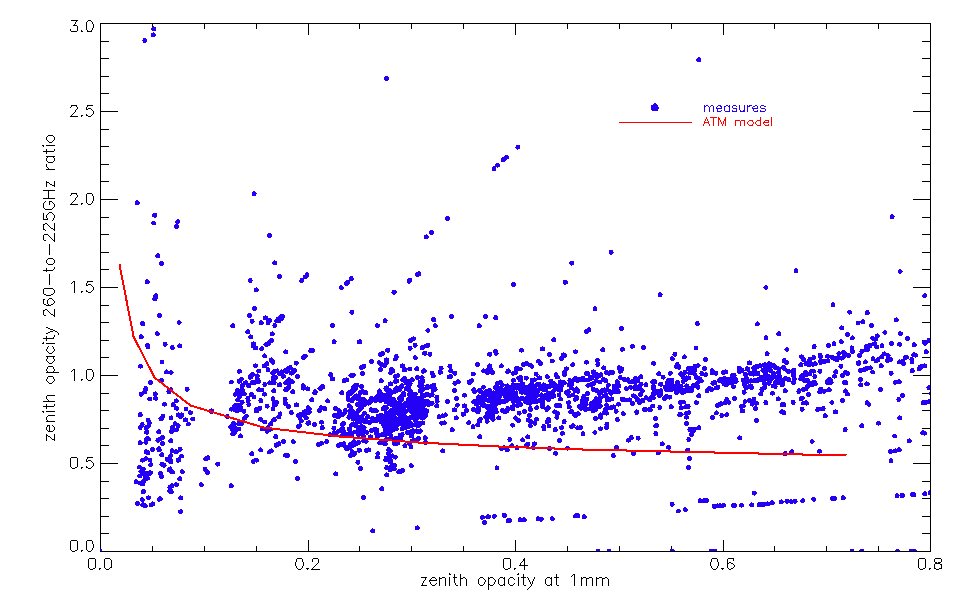
\includegraphics[width=0.65\textwidth]{Figures/opacity_tau2_tau225_ratio_N2R9_N2R10.png}
\caption{Ratios between the 150 GHz and the 260 GHz NIKA2 zenith opacity
estimates and between the NIKA2 $\tau$ and the IRAM taumeter
values. The expectation values derived for NIKA2 bands
using the ATM model described in \ref{Pardo2002} are shown for
comparison (red and orange curves).}
  \label{fig:opacity_ratios}
\end{center}
\end{figure}

\begin{figure}[ht]
\begin{center}
  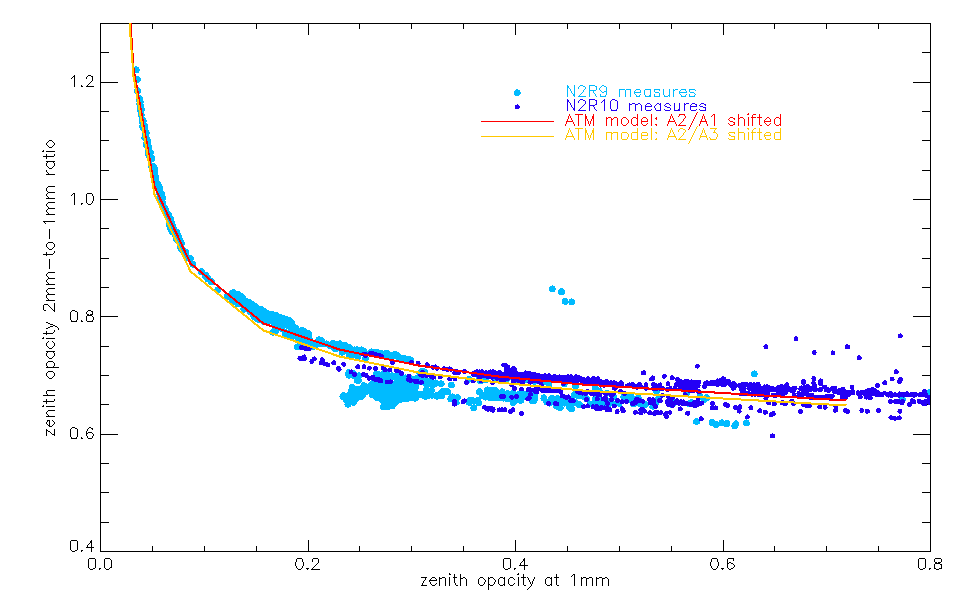
\includegraphics[width=0.8\textwidth]{Figures/opacity_tau1_tau2_byrun_ratio_N2R9_N2R10.png}
  \caption{Ratio between the 150 GHz and the 260 GHz NIKA2 zenith opacity
estimates. The expectation values derived for NIKA2 bands
using the ATM model described in \ref{Pardo2002} are shown for
comparison (red and orange curves). The observed NIKA2 opacity ratio
has a smooth, consistent behaviour over the overall probed opacity range,
and very few outlier estimates are seen although no scan selection has
been performed (out from discarding the dark tests). Also remarkable
is the consistency between estimates obtained during two campaigns
held two months apart in different weather conditions (good to average
during N2R9 and poor and often hightly unstable conditions during
N2R10). Some sub-structures are seen in the opacity ratio, which are
under investigations. They can have several origins (telescope cabin
temperature variation, variation of the $0_2$ fraction, atmospheric
temperature variation, internal temperature variations, etc).  
  }
  \label{fig:opacity_ratio_perrun}
\end{center}
\end{figure}


\begin{figure}[ht]
\begin{center}
  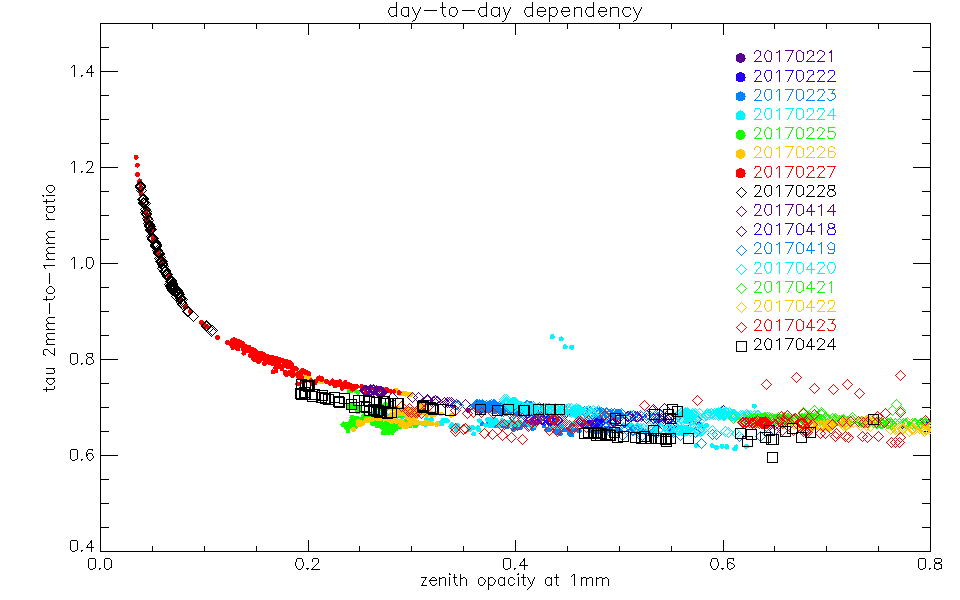
\includegraphics[width=0.8\textwidth]{Figures/opacity_tau1_tau2_ratio_perday_N2R9_N2R10.png}
  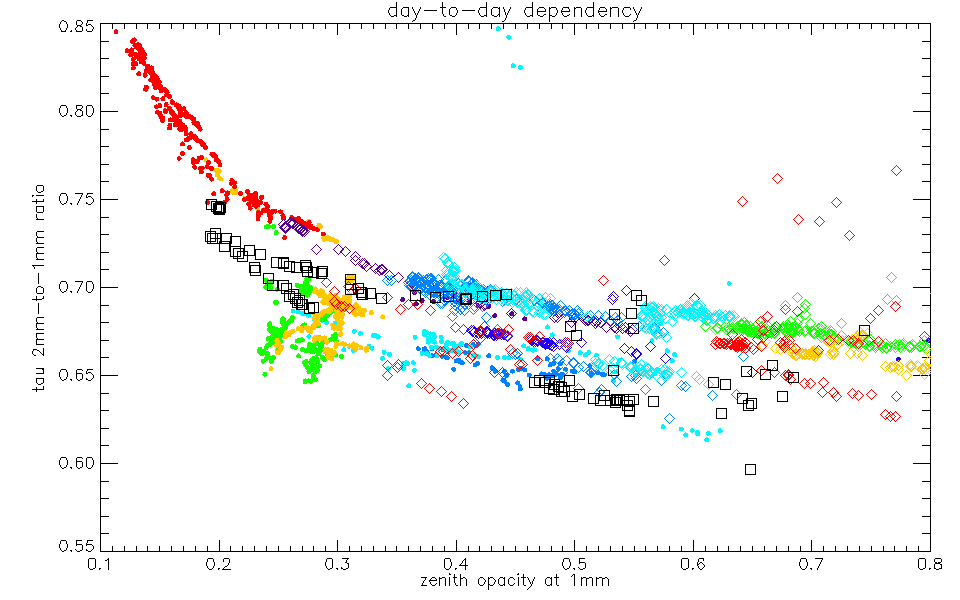
\includegraphics[width=0.8\textwidth]{Figures/opacity_tau1_tau2_ratio_perday_zoom_N2R9_N2R10.png}
  \caption{Ratio between the 150 GHz and the 260 GHz NIKA2 zenith
    opacity estimates. The 4 outlier estimates on February, 24 (in
    cyan) correspond to a test using the external
    calibrator. Different regimes are seen on the 25th and 26th of
    February, while the weather conditions were too unstable to allow
    the astronomer team to focus.
  }
  \label{fig:opacity_ratio_perday}
\end{center}
\end{figure}


\begin{figure}[ht]
\begin{center}
  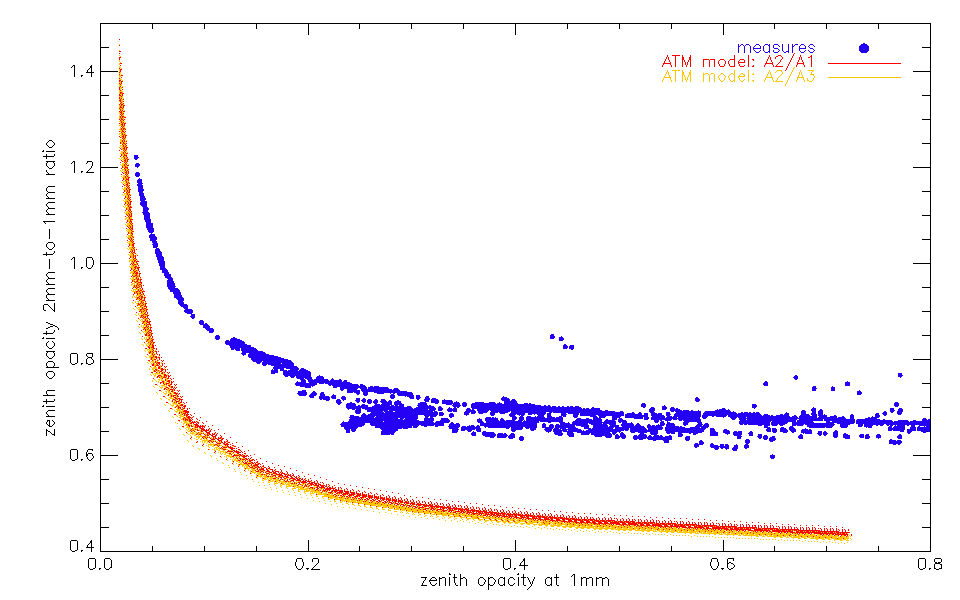
\includegraphics[width=0.8\textwidth]{Figures/opacity_tau1_tau2_ratio_bperror10pc_N2R9_N2R10.png}
  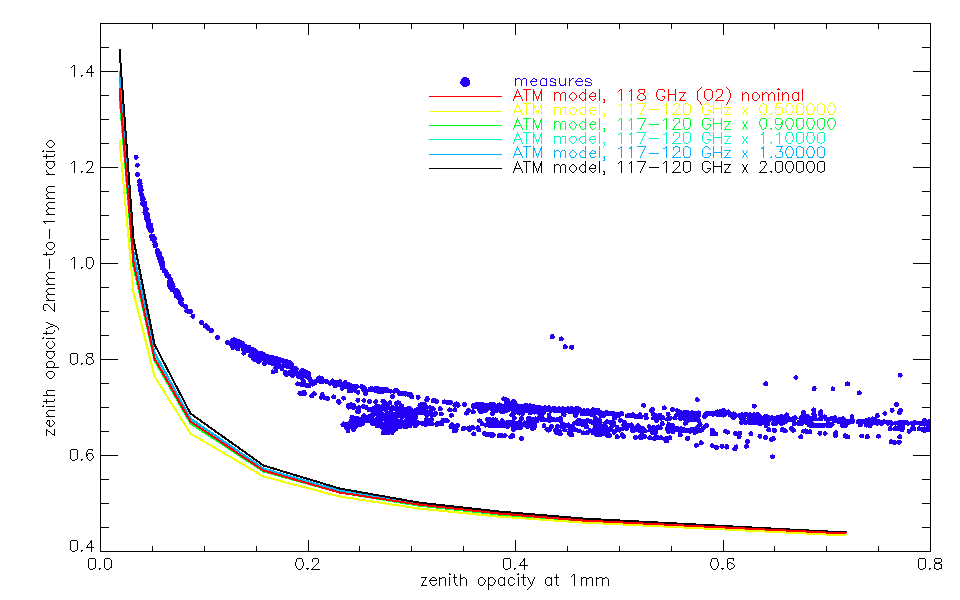
\includegraphics[width=0.8\textwidth]{Figures/opacity_tau1_tau2_ratio_o2fraction_N2R9_N2R10.png}
\caption{Uncertainty of NIKA2 $\tau$ values. Upper panel: The impact
  of the NIKA2 transmission measurement uncertainties is illustrated
  using a very pessimistic relative uncertainty of $10\%$ (instead of
  the more realistic $1\%$ errors). Lower panel: The impact of the
uncertainty on the atmospheric absorption around $118\, \rm{GHz}$, due
to the lack of precise knowledge of the fraction of oxygene in the
atmosphere. The nominal absorption predicted by the ATM model is
modified by a factor from 0.5 to 2 in the $117-120\, \rm{GHz}$
frequency band, where the $0_2$ contributions largely dominates the
water vapor ones. }
  \label{fig:opacity_errors}
\end{center}
\end{figure}

\begin{figure}[ht]
\begin{center}
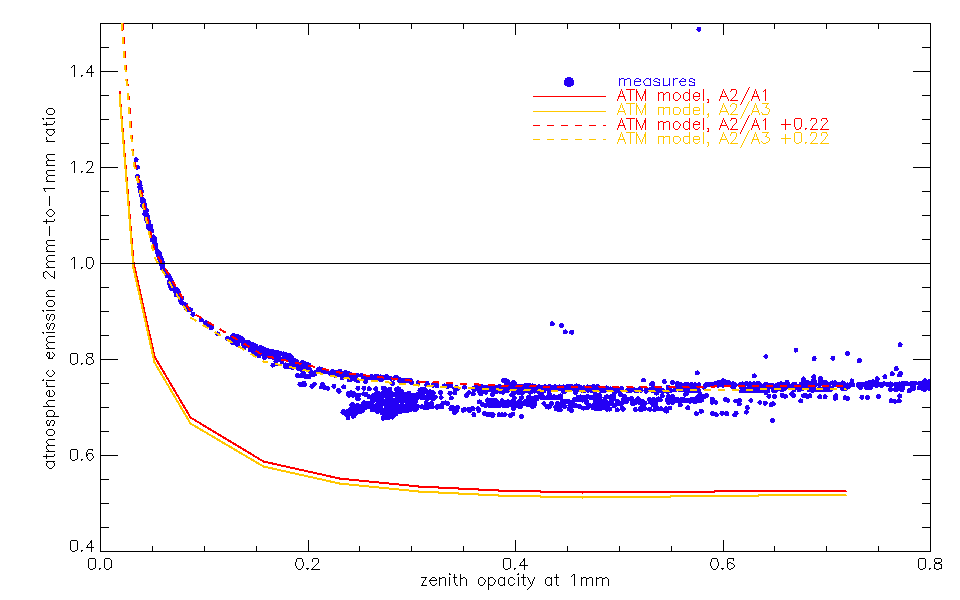
\includegraphics[width=0.9\textwidth]{Figures/opacity_tau1_tau2_emissionratio_N2R9_N2R10.png}
\caption{Ratio of the atmospheric emission in NIKA2 bands defined as
  in Eq.~\ref{eq:opacity_emission_ratio}, compared with the ATM-model
  predicted ratio calculated as in Eq.~\ref{eq:opacity_emission_ratio_model}}
  \label{fig:opacity_emission}
\end{center}
\end{figure}

The ratios between the 150 GHz and the 260 GHz NIKA2 zenith opacity
estimates, quoted $\tau_{2mm}$ and $\tau_{1mm}$ , and
between the NIKA2 $\tau$ and the IRAM taumeter values are presented in
Fig.~\ref{opacity_ratios}, along with the expectation values derived for NIKA2 bands
using the ATM model described in \ref{Pardo2002}. Namely, these
predicted values $\tau^{th}$ are calculated from the ATM-model
atmospheric zenith opacity $\tau^{ATM}$ using:  
\begin{equation}
  \tau^{th}_{A_i} = - \ln{\frac{\int e^{-\tau^{ATM}(\nu)}
      T_{A_i}(\nu) d\nu}{ \int T_{A_i}(\nu) d\nu}},
\end{equation}

where the NIKA2 bandpasses $T_{A_i}$ for arrays $A_i$, $i=1, 2, 3$, are the Martin-Pupplet reference transmissions
corrected by a Rayleigh-Jeans term  $T'_{A_i}(\nu) /
\left( \frac{\nu}{\nu_0}\right)^2$. 

In Fig.~\ref{fig:opacity_emission}, we
show the ratio of the atmospheric emission in NIKA2 bands defined as:
\begin{equation}
  R_{\rm{atm}} = \frac{1-e^{-\tau_{2mm}}}{1-e^{-\tau_{1mm}}}.
    \label{eq:opacity_emission_ratio}
\end{equation}

It is compared with the ATM-model predicted ratio
\begin{equation}
  R_{\rm{atm}}^{th} = \frac{\int (1 - e^{-\tau^{\rm{ATM}}}) T_{A_2}(\nu) d\nu }{\int T_{A_2}(\nu) d\nu} / \frac{\int (1 -
      e^{-\tau^{\rm{ATM}}}) T_{A_{1}}(\nu) d\nu }{\int T_{A_1}(\nu)
        d\nu} .
      \label{eq:opacity_emission_ratio_model}
\end{equation}

In Fig.~\ref{fig:opacity_errors}, we investigate different effects that can impact the precision with
which the zenith opacities are determined: the upper panel shows the
expected dispersion in the NIKA2 $\tau$ values coming from the transmission
measurement uncertainties: to higlight this effect, we consider a very
pessimistic relative uncertainty of $10\%$ (whereas $1\%$ would have
been a more realistic value), and the lower panel shows the impact of the
uncertainty on the fraction of oxygene in the atmosphere, which mainly 
translates in an uncertainty on the atmospheric absorption around
$118\, \rm{GHz}$: the nominal absorption predicted by the ATM model is
modified by a factor from 0.5 to 2 in the $117-120\, \rm{GHz}$
frequency band, where the $0_2$ contributions largely dominates the
water vapor ones. 



We have compared $C_0$ values, the resonance frequency at zero atmosphere,
between different runs. It appears to vary in a systematic manner. For example
we have compared N2R6 and N2R7. The change of frequencies when converted to
temperature (with $c_1$) is of about $25$ and $86$~K at 1 and $2$~mm. This
cannot be a real change of the background. Translated back by a median value
of $c_1$ ($=2500$ and $1500$~Hz/K at 1 and 2 mm), we obtain a 62.5 and 128 kHz
median downward shift of all resonant frequencies between N2R6 (October 2016)
and N2R7 (December 2016). The likely explanation is that of a slight ageing of
the KIDs. A single monolayer of oxyde could be enough to produce the downward
shift.



% LP: copie de l'intro de Xavier
In NIKA2, the opacity is measured via a total-power technique, which was
successfully tested with NIKA. The details of this technique and its agreement
with the Atmospheric Transmission at Microwaves (ATM) model
(\cite{2001IEEE....49.1683C}) are described in \cite{Catalano:2014nml}. The
underlying idea is to replace the opacity, usually delivered by the resident
IRAM tau-meter that performs elevation scans at a fixed azimuth and is
operating at 225\,GHz, by a measurement that uses the NIKA2 instrument itself
as a tau-meter. Using this procedure we can directly derive an opacity
integrated in the NIKA2 very bandpasses and in the same line-of-sight of the
source in the considered map. For that purpose, we assume that the resonance
frequency of each KID varies linearly with the total power. First, we have to
calibrate the relationship between total power and opacity. Then we can use
that calibration to measure the opacity during a given scan.
% fin copie


%----------------------------------------------------------------------------------------
%	Method
%----------------------------------------------------------------------------------------
\subsection{Methodology}
For each kid $k$, the absolute value of the resonance frequency
$f_{tone}^k$ moves with the atmospheric load according to

\begin{equation}
f_{tone}^k = C_0^k - C_1^k T_{atm}[1-e^{-\tau/\sin\delta}]
\end{equation}

%FXD corrected 
%{\bf LP: pourquoi signe plus alors qu'on utilise un signe moins dans
%  Eq. 2 du papier instru ?}

where $C_0^k$ is a constant equal to the resonance
frequency at zero opacity, $C_1^k$ is the calibration conversion
factor in kHz$/$K, $T_{atm}$ is the equivalent temperature
of the atmosphere (taken as a constant at 270K), $\tau$ the zenith
opacity and $\delta$ the average elevation of the telescope.
By assuming a homogeneous plane-parallel atmosphere, the airmass $x$ is defined from the
elevation as $x = \sin\delta$. 

The coefficients $C_0^k$ and $C_1^k$ are expected to be constant in time
within at least a cooldown cycle, and are determined using a {\tt
  skydip} procedure. This consists in moving
the telescope in elevation step by step and monitoring, for each kid, the
evolution of $f_{tone}^k$ versus the air mass and to fit the zenith opacity $\tau$ and
$C_0^k$ and $C_1^k$. During a {\tt skydip}, the telescope performs
eleven  steps in the elevation range from 19 to 65 degrees, regularly
spaced in airmass. For each step, we acquire about twenty seconds of
time traces to reduce the error in the determination of $f_{tone}^k$.

All skydips, obtained under various opacity
conditions, are analysed together to break the degeneracies between
the opacity and the responsivity ($C_1^k$). The procedure has two steps.
First, all the skydips are analysed individually to simply extract
$f_{tone}^k$ for each stable elevation. Secondly, a simultaneous fit is done
for all 
parameters ($\tau$, $C_0^k$ and $C_1^k$.)
Error bars on $\tau$ are estimated by doing
this procedure on blocks of 40 kids only and getting a dispersion on the
resulting $\tau$ from the different blocks. Usually the dispersion comes out as
$4\times 10^{-3}$ at 1 mm and $1\times 10^{-3}$ at 2 mm. Once the $\tau$ values
are estimated for each skydip (as the average over the blocks), we compute
(while fixing $\tau$) the $C_0$ and $C_1$ final values for each KID. We thus
retrieve the coefficients of all the KIDs even though some of them could not
contribute to the $\tau$ determination.


%----------------------------------------------------------------------------------------
%	Tests
%----------------------------------------------------------------------------------------
\subsection{Opacity measurement consistency tests}

%{\bf copy from the 'Instru' paper}

\begin{figure}[ht]
\begin{center}
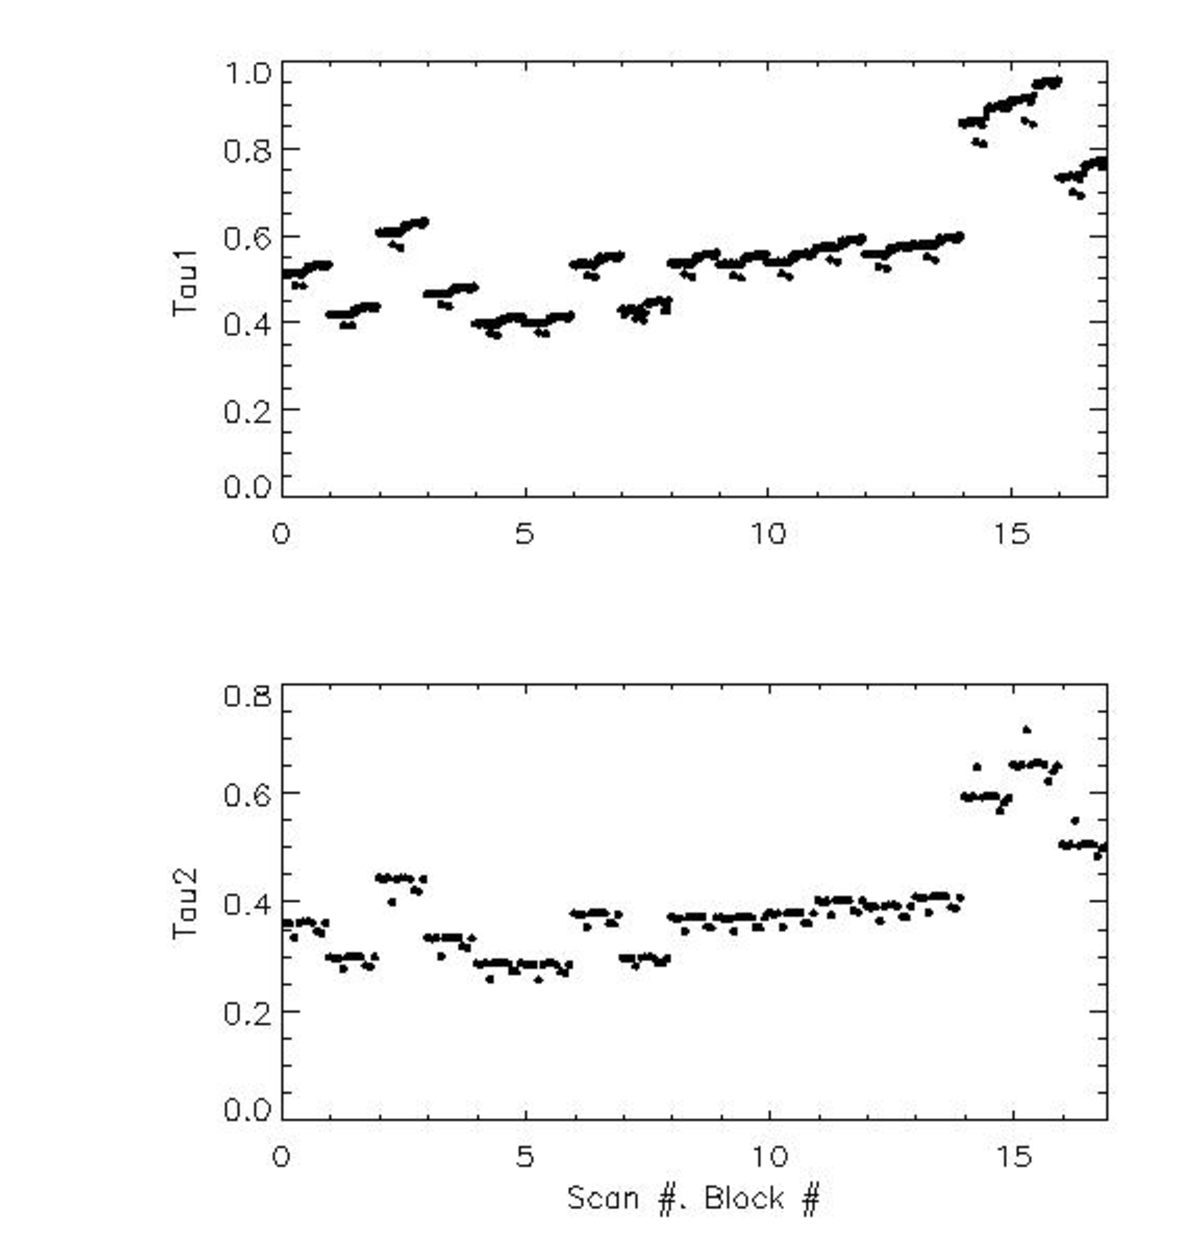
\includegraphics[scale=0.8]{Figures/test_allskd_N2R10v3commiss2.pdf}
\caption{Atmospheric opacity as measured from the NIKA2 data 
at 260 (top) and 150\,GHz (bottom) during N2R10
commissioning campaign. Each block of 40 KIDs gives an independent estimate of
the opacity value for each skydip scan (the integer abscissae). The block
number is the decimal value of the abscissae.
\label{fig:taumeas_paper}}
\end{center}
\end{figure}

\begin{figure}[ht]
\begin{center}
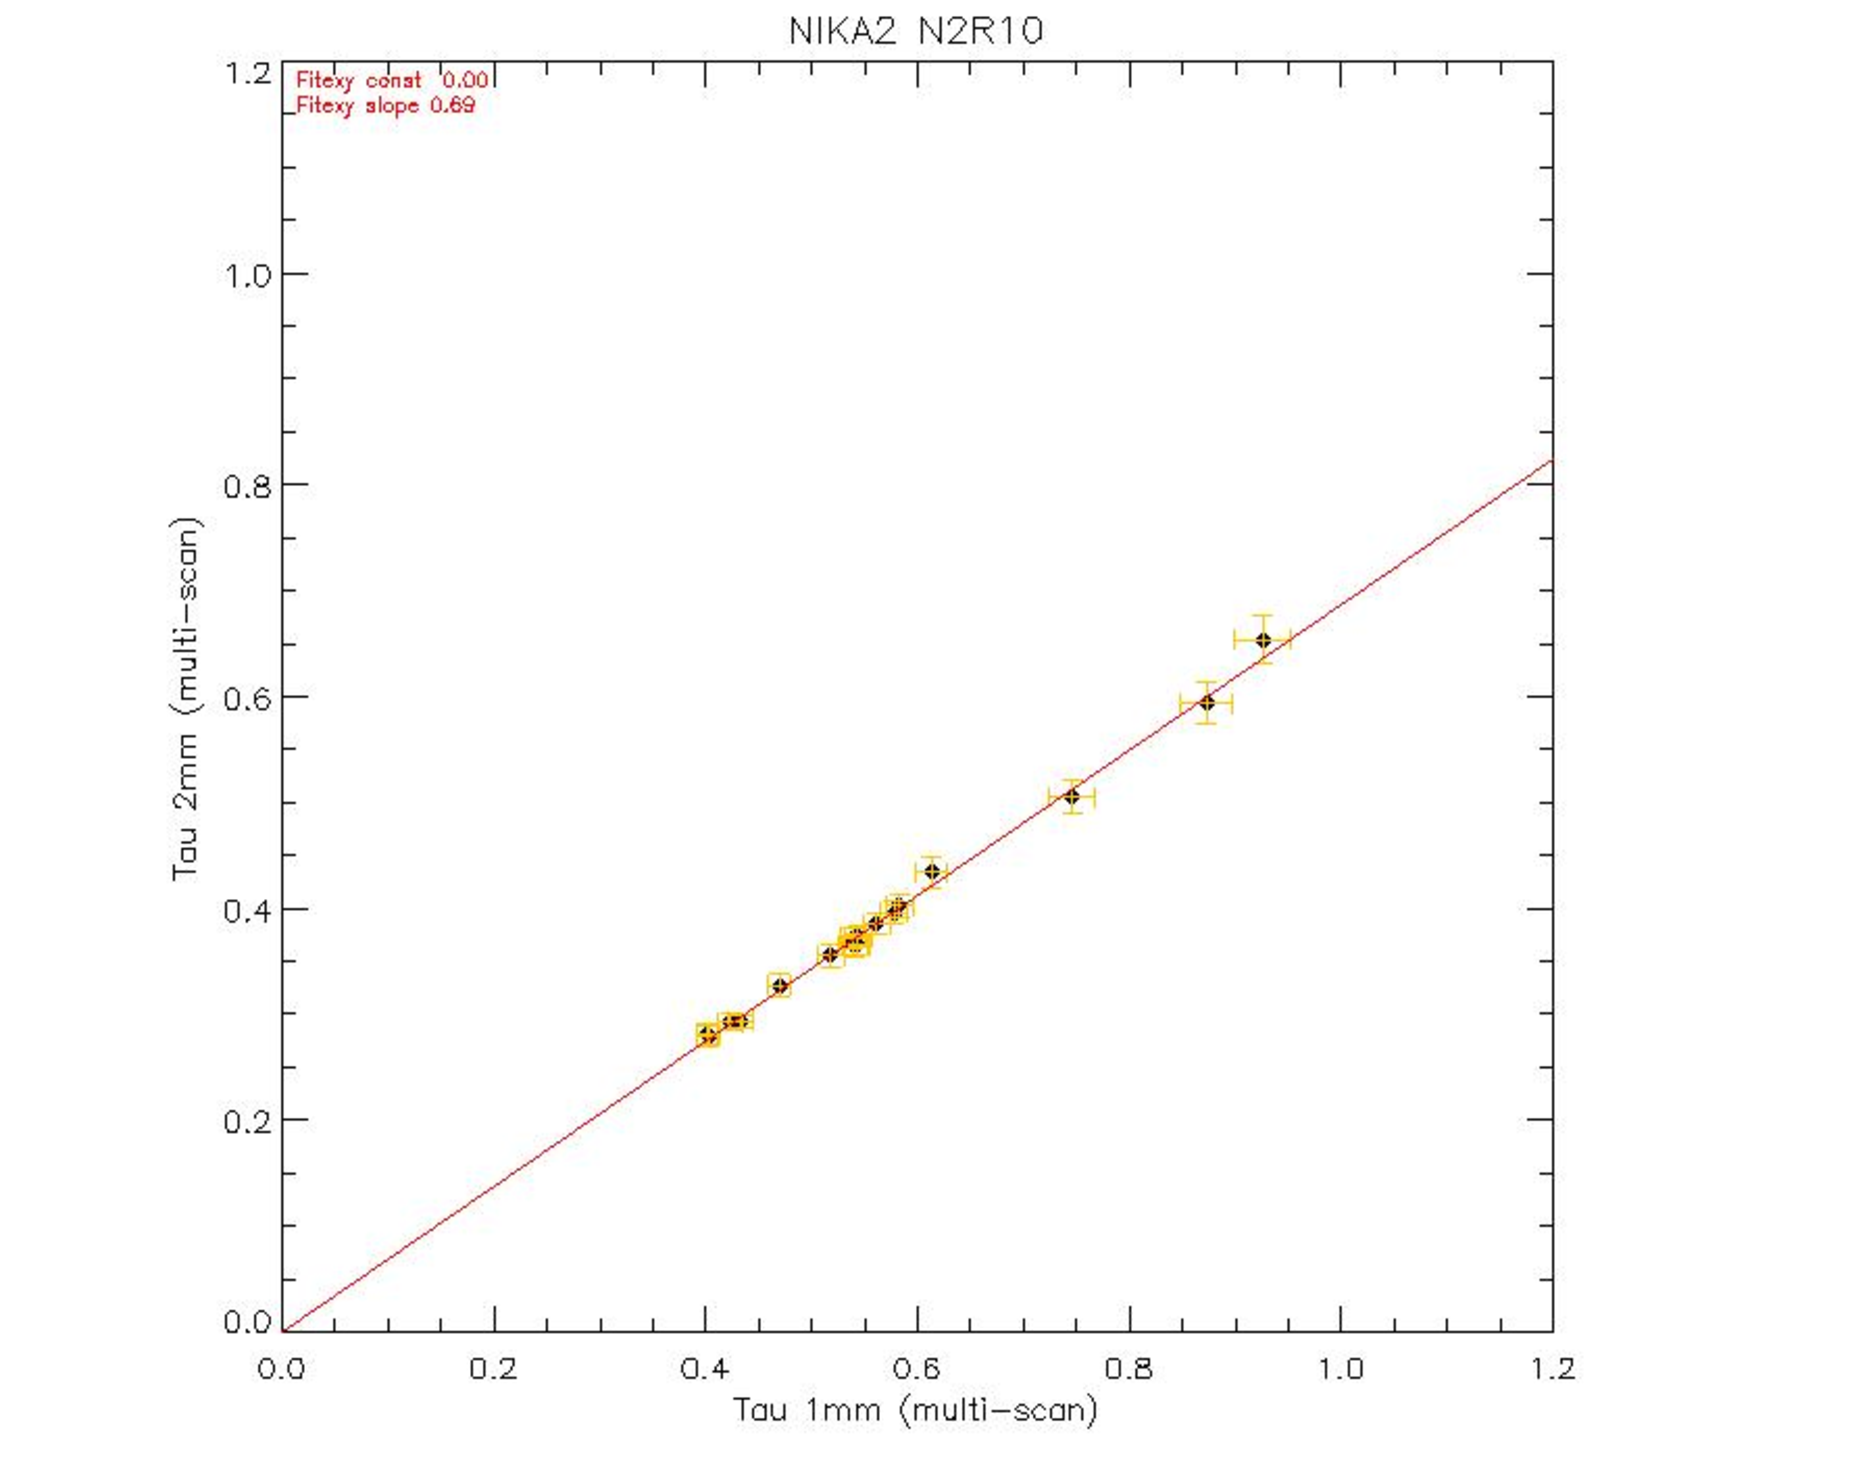
\includegraphics[scale=0.8]{Figures/test_allskd_N2R10v2commiss1.pdf}
\caption{Atmospheric opacity as measured from the NIKA2 data 
at 260 and 150\,GHz during N2R10
commissioning campaign. The error bars are in fact dispersion of the deduced
opacities between blocks of 40 KIDs.
\label{fig:taumeas_paper}}
\end{center}
\end{figure}

We observe that the skydip-fitted $\tau$ values are, as expected, common
between different detectors of the same array (the two 1mm arrays show
slightly different values). By comparing the results of different skydips, we
have verified experimentally that the coefficients $C_0$, $C_1$ are stable,
within the fit errors, on very long time scales within a cooldown cycle. The
coefficients can thus be applied to the whole observing campaign in order to
recover the opacity of each scan.


% \noindent {\bf FM : a figure would help to convince the reader that it is stable on lng time
% scale, which is a key point.}\\ FXD: I will do that figure


\begin{figure}[ht]
\begin{center}
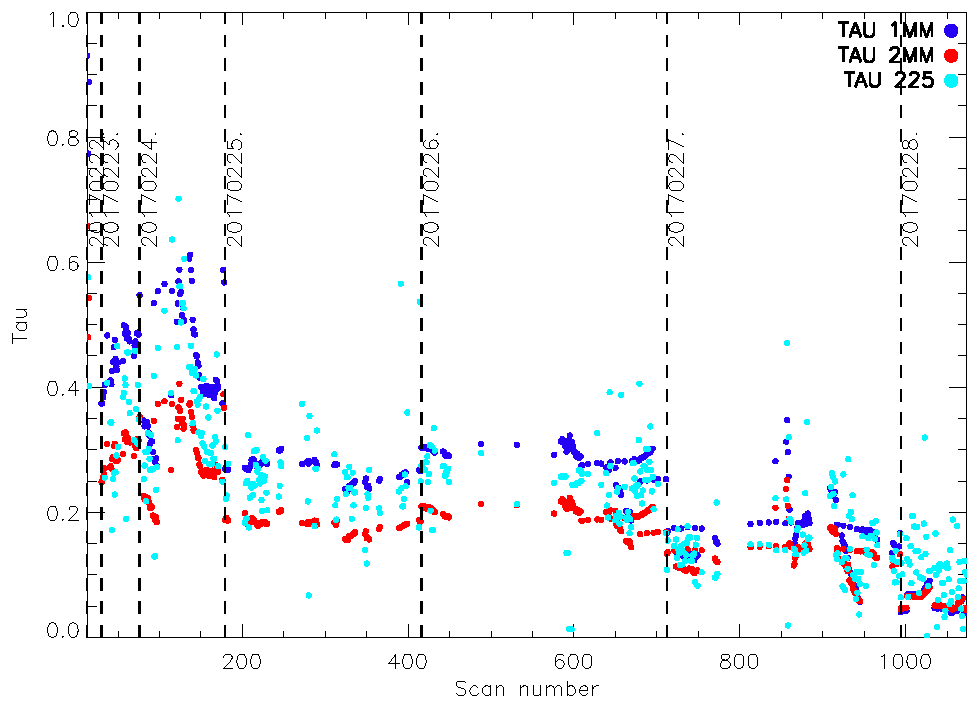
\includegraphics[scale=0.8]{../../Paper_NIKA2_Technical/opacity_evol_run22.pdf}
\caption{Atmospheric opacity as measured from the IRAM 225\,GHz taumeter
(cyan), and from the NIKA2 data at 150 (red) and 260\,GHz (blue) during N2R9
commissioning campaign (Feb. 2017). We stress the fact that the IRAM 225\,GHz
taumeter data is not used for the atmospheric correction and is plotted here
just for comparison.
  \label{fig:taumeas_paper}}
\end{center}
\end{figure}


\begin{figure}[ht]
\begin{center}
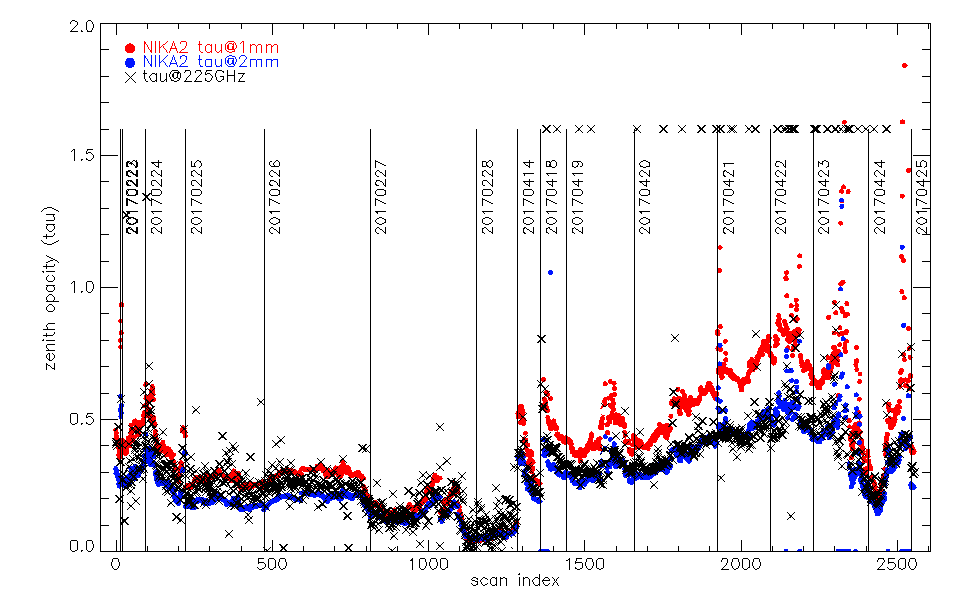
\includegraphics[width=\linewidth]{Figures/opacity_vs_index_N2R9_N2R10.png}
\caption{Atmospheric opacity as measured from the IRAM 225\,GHz
  taumeter (black crosses), and from the NIKA2 data at 150 (red) and 260\,GHz (blue) during 
  N2R9 and N2R10 commissioning campaigns.  We stress the fact that the IRAM 225\,GHz taumeter data is not used for the atmospheric correction and is plotted here just for comparison.
  \label{fig:taumeas}}
\end{center}
\end{figure}


In Fig.~\ref{fig:taumeas} {\bf(and Fig.~\ref{fig:taumeas_paper} of
  \ref{NIKA2-Tech}) } we present the evolution of the NIKA2 in-band
opacities for all the 'OTF' scans (about 1300 scans per runs) of the
N2R9 run held in February and the N2R10 run in April 2017. These are
compared to the IRAM tau-meter values. We observe an agreement on the global trend between the IRAM tau-meter opacity
(225 GHz) and the NIKA2 values. These latter show, however,
a smaller dispersion (less than one percent).
% {\bf FM : how small ?}.


We find an average ratio between the 150 GHz and the 260 GHz NIKA2 values of
about 0.6, a bit higher than ATM model expectations. We notice however that
the 150 GHz-to-260 GHz opacity ratio varies significantly for opacities (at
150 GHz) below 0.2. This effect is likely to be linked to an $O_2$ atmospheric
line which becomes saturated or to some spillover at 2mm. This point is,
however, still under investigation.''


% \noindent {\bf FM : a figure of the ratio of taus would be useful. It should be compared with  
% Fig. \ref{thopacities}, which should appear in this section ...}
% FXD: figure above gives the measured ratio. 


\begin{figure}[ht]
\begin{center}
  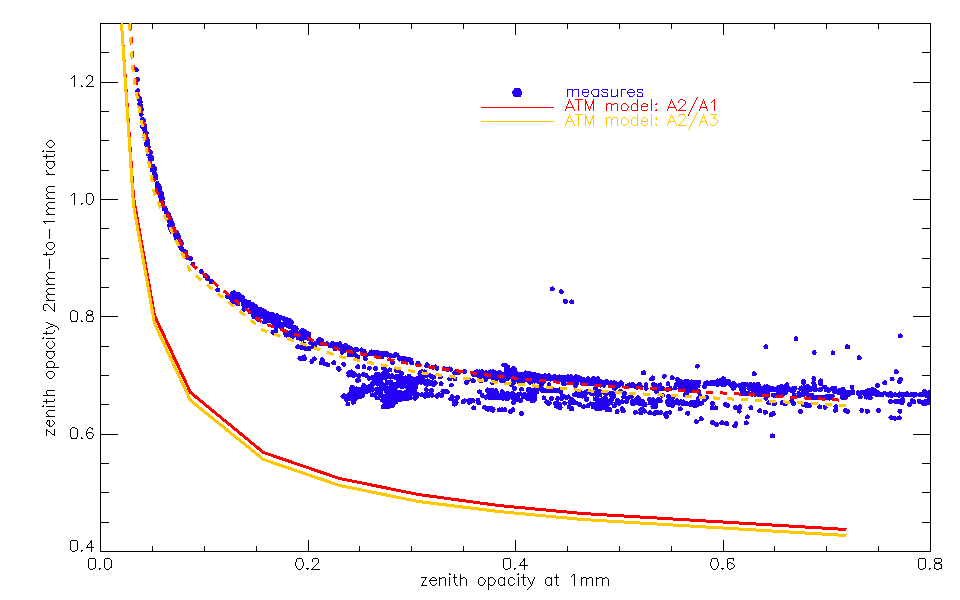
\includegraphics[width=0.65\textwidth]{Figures/opacity_tau1_tau2_ratio_N2R9_N2R10.png}
  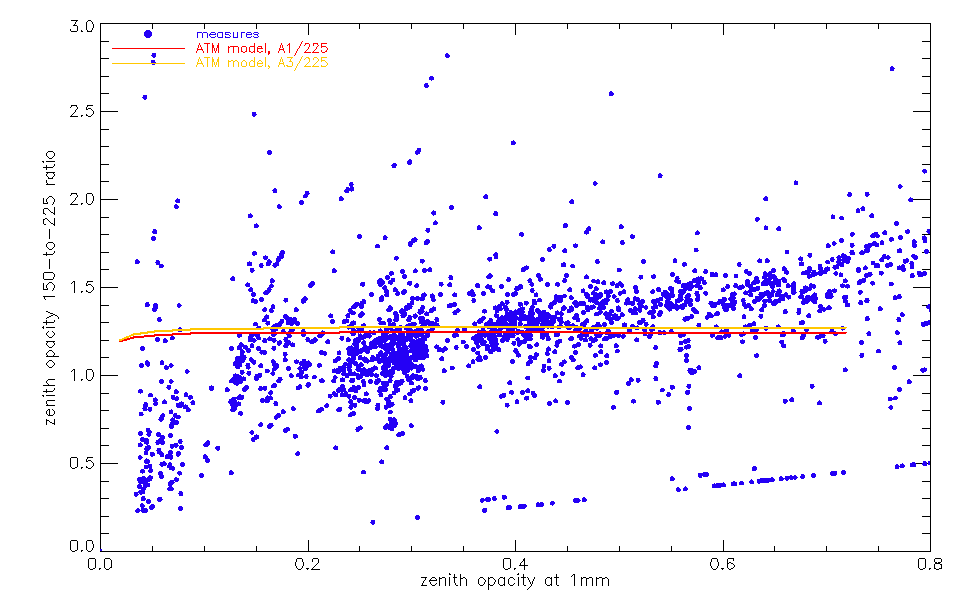
\includegraphics[width=0.65\textwidth]{Figures/opacity_tau1_tau225_ratio_N2R9_N2R10.png}
  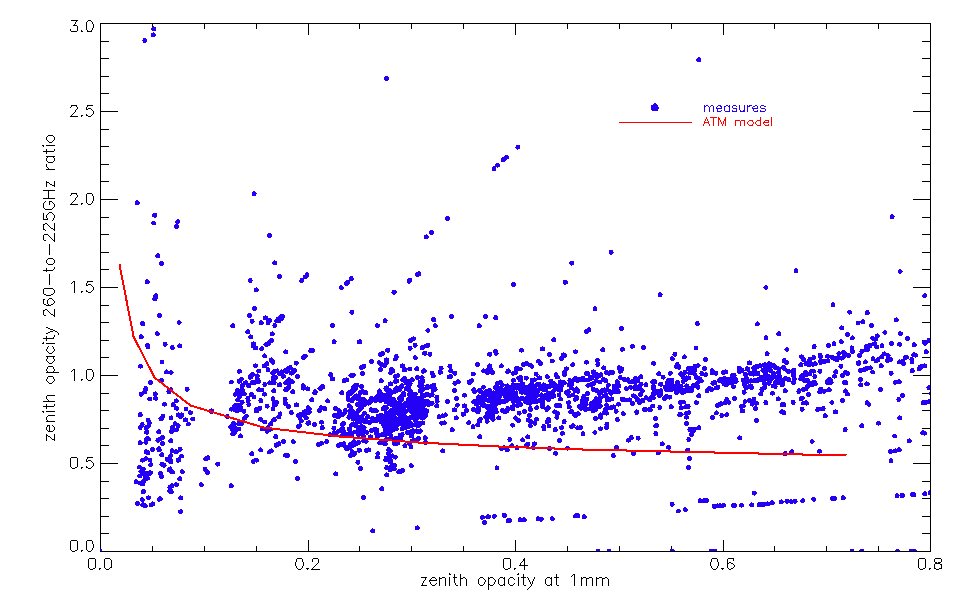
\includegraphics[width=0.65\textwidth]{Figures/opacity_tau2_tau225_ratio_N2R9_N2R10.png}
\caption{Ratios between the 150 GHz and the 260 GHz NIKA2 zenith opacity
estimates and between the NIKA2 $\tau$ and the IRAM taumeter
values. The expectation values derived for NIKA2 bands
using the ATM model described in \ref{Pardo2002} are shown for
comparison (red and orange curves).}
  \label{fig:opacity_ratios}
\end{center}
\end{figure}

\begin{figure}[ht]
\begin{center}
  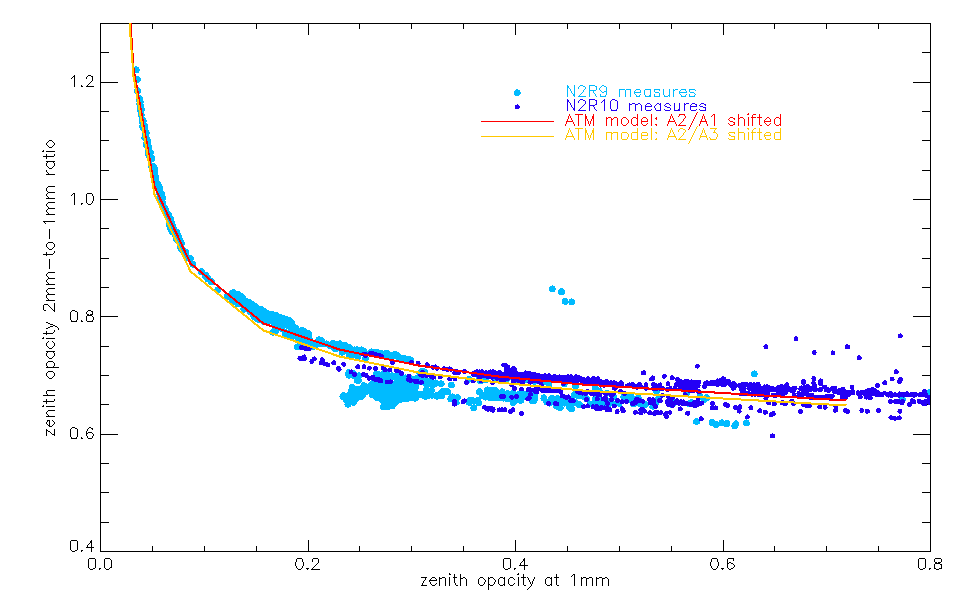
\includegraphics[width=0.8\textwidth]{Figures/opacity_tau1_tau2_byrun_ratio_N2R9_N2R10.png}
  \caption{Ratio between the 150 GHz and the 260 GHz NIKA2 zenith opacity
estimates. The expectation values derived for NIKA2 bands
using the ATM model described in \ref{Pardo2002} are shown for
comparison (red and orange curves). The observed NIKA2 opacity ratio
has a smooth, consistent behaviour over the overall probed opacity range,
and very few outlier estimates are seen although no scan selection has
been performed (out from discarding the dark tests). Also remarkable
is the consistency between estimates obtained during two campaigns
held two months apart in different weather conditions (good to average
during N2R9 and poor and often hightly unstable conditions during
N2R10). Some sub-structures are seen in the opacity ratio, which are
under investigations. They can have several origins (telescope cabin
temperature variation, variation of the $0_2$ fraction, atmospheric
temperature variation, internal temperature variations, etc).  
  }
  \label{fig:opacity_ratio_perrun}
\end{center}
\end{figure}


\begin{figure}[ht]
\begin{center}
  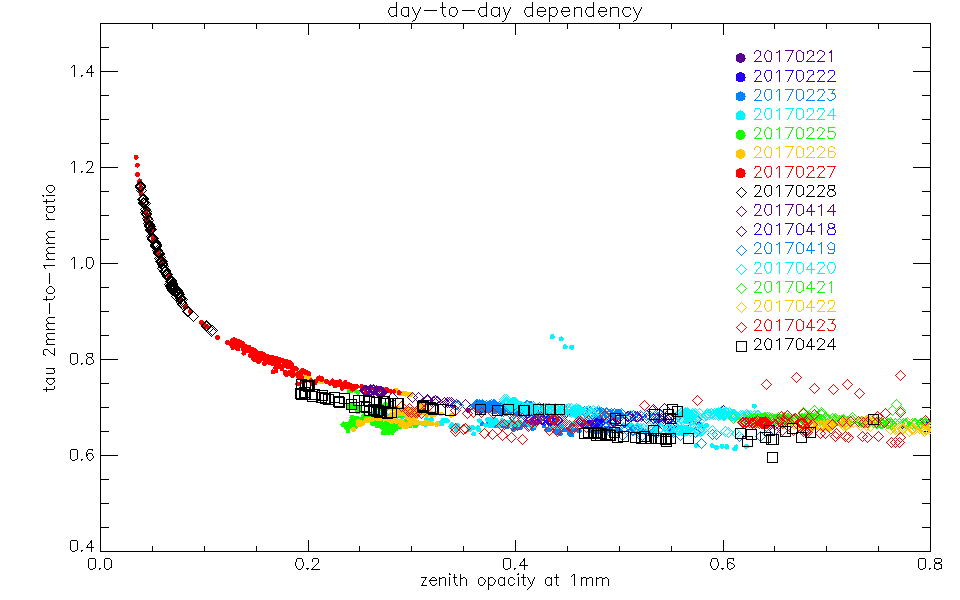
\includegraphics[width=0.8\textwidth]{Figures/opacity_tau1_tau2_ratio_perday_N2R9_N2R10.png}
  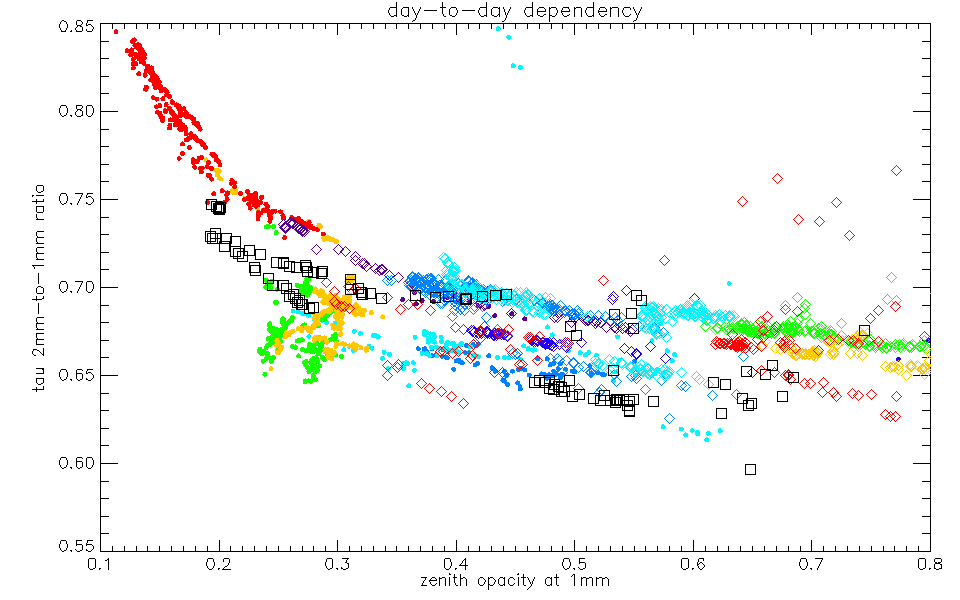
\includegraphics[width=0.8\textwidth]{Figures/opacity_tau1_tau2_ratio_perday_zoom_N2R9_N2R10.png}
  \caption{Ratio between the 150 GHz and the 260 GHz NIKA2 zenith
    opacity estimates. The 4 outlier estimates on February, 24 (in
    cyan) correspond to a test using the external
    calibrator. Different regimes are seen on the 25th and 26th of
    February, while the weather conditions were too unstable to allow
    the astronomer team to focus.
  }
  \label{fig:opacity_ratio_perday}
\end{center}
\end{figure}


\begin{figure}[ht]
\begin{center}
  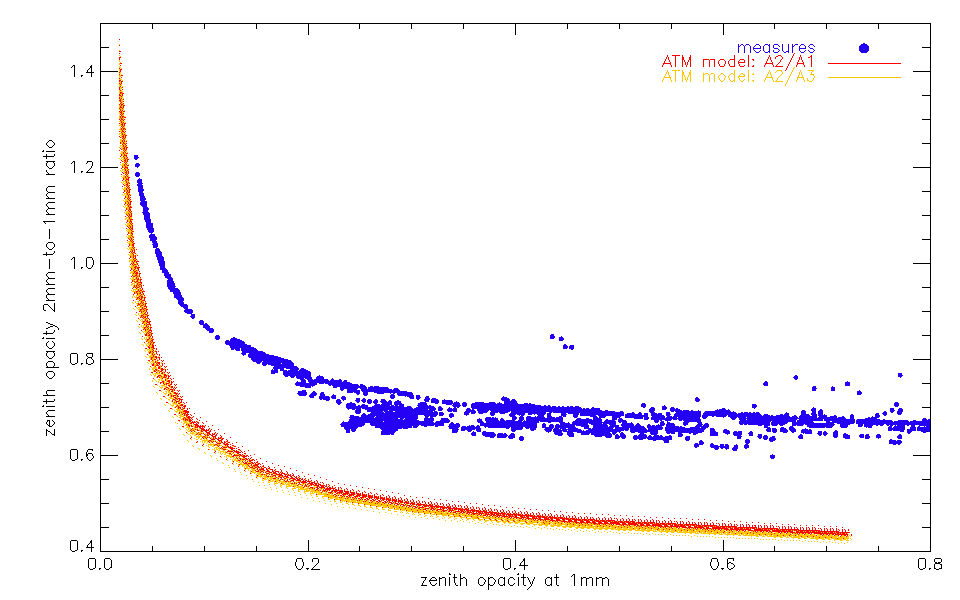
\includegraphics[width=0.8\textwidth]{Figures/opacity_tau1_tau2_ratio_bperror10pc_N2R9_N2R10.png}
  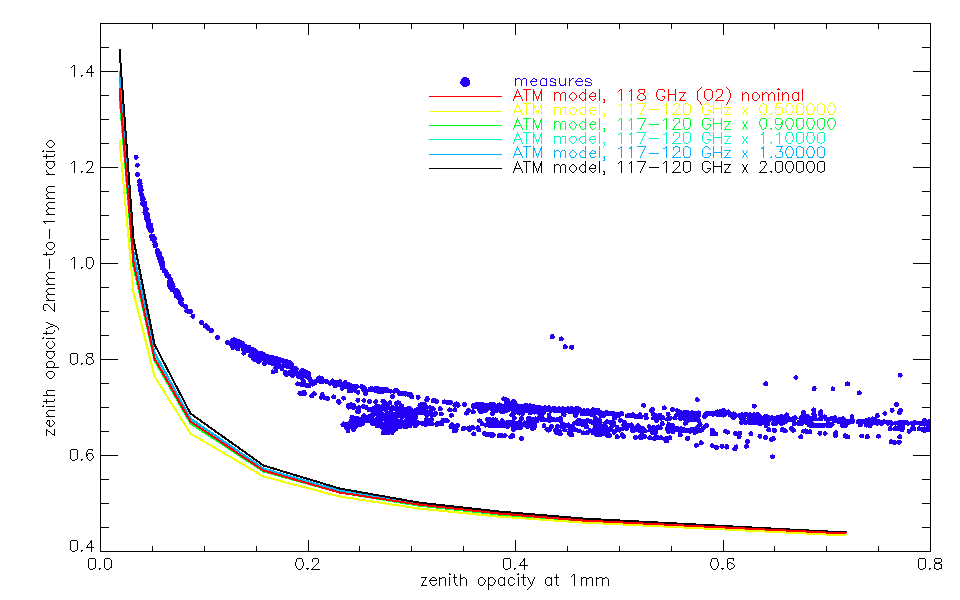
\includegraphics[width=0.8\textwidth]{Figures/opacity_tau1_tau2_ratio_o2fraction_N2R9_N2R10.png}
\caption{Uncertainty of NIKA2 $\tau$ values. Upper panel: The impact
  of the NIKA2 transmission measurement uncertainties is illustrated
  using a very pessimistic relative uncertainty of $10\%$ (instead of
  the more realistic $1\%$ errors). Lower panel: The impact of the
uncertainty on the atmospheric absorption around $118\, \rm{GHz}$, due
to the lack of precise knowledge of the fraction of oxygene in the
atmosphere. The nominal absorption predicted by the ATM model is
modified by a factor from 0.5 to 2 in the $117-120\, \rm{GHz}$
frequency band, where the $0_2$ contributions largely dominates the
water vapor ones. }
  \label{fig:opacity_errors}
\end{center}
\end{figure}

\begin{figure}[ht]
\begin{center}
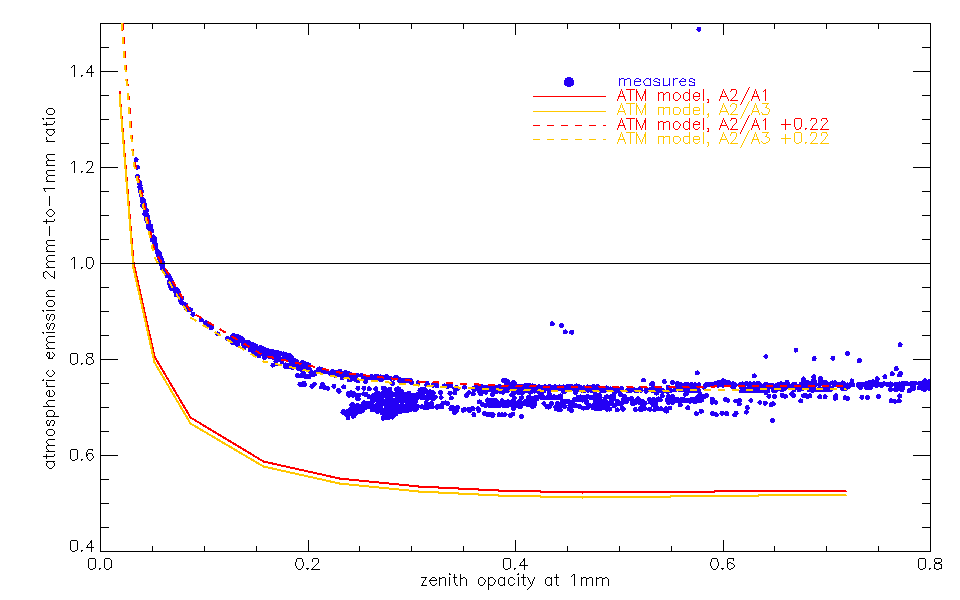
\includegraphics[width=0.9\textwidth]{Figures/opacity_tau1_tau2_emissionratio_N2R9_N2R10.png}
\caption{Ratio of the atmospheric emission in NIKA2 bands defined as
  in Eq.~\ref{eq:opacity_emission_ratio}, compared with the ATM-model
  predicted ratio calculated as in Eq.~\ref{eq:opacity_emission_ratio_model}}
  \label{fig:opacity_emission}
\end{center}
\end{figure}

The ratios between the 150 GHz and the 260 GHz NIKA2 zenith opacity
estimates, quoted $\tau_{2mm}$ and $\tau_{1mm}$ , and
between the NIKA2 $\tau$ and the IRAM taumeter values are presented in
Fig.~\ref{opacity_ratios}, along with the expectation values derived for NIKA2 bands
using the ATM model described in \ref{Pardo2002}. Namely, these
predicted values $\tau^{th}$ are calculated from the ATM-model
atmospheric zenith opacity $\tau^{ATM}$ using:  
\begin{equation}
  \tau^{th}_{A_i} = - \ln{\frac{\int e^{-\tau^{ATM}(\nu)}
      T_{A_i}(\nu) d\nu}{ \int T_{A_i}(\nu) d\nu}},
\end{equation}

where the NIKA2 bandpasses $T_{A_i}$ for arrays $A_i$, $i=1, 2, 3$, are the Martin-Pupplet reference transmissions
corrected by a Rayleigh-Jeans term  $T'_{A_i}(\nu) /
\left( \frac{\nu}{\nu_0}\right)^2$. 

In Fig.~\ref{fig:opacity_emission}, we
show the ratio of the atmospheric emission in NIKA2 bands defined as:
\begin{equation}
  R_{\rm{atm}} = \frac{1-e^{-\tau_{2mm}}}{1-e^{-\tau_{1mm}}}.
    \label{eq:opacity_emission_ratio}
\end{equation}

It is compared with the ATM-model predicted ratio
\begin{equation}
  R_{\rm{atm}}^{th} = \frac{\int (1 - e^{-\tau^{\rm{ATM}}}) T_{A_2}(\nu) d\nu }{\int T_{A_2}(\nu) d\nu} / \frac{\int (1 -
      e^{-\tau^{\rm{ATM}}}) T_{A_{1}}(\nu) d\nu }{\int T_{A_1}(\nu)
        d\nu} .
      \label{eq:opacity_emission_ratio_model}
\end{equation}

In Fig.~\ref{fig:opacity_errors}, we investigate different effects that can impact the precision with
which the zenith opacities are determined: the upper panel shows the
expected dispersion in the NIKA2 $\tau$ values coming from the transmission
measurement uncertainties: to higlight this effect, we consider a very
pessimistic relative uncertainty of $10\%$ (whereas $1\%$ would have
been a more realistic value), and the lower panel shows the impact of the
uncertainty on the fraction of oxygene in the atmosphere, which mainly 
translates in an uncertainty on the atmospheric absorption around
$118\, \rm{GHz}$: the nominal absorption predicted by the ATM model is
modified by a factor from 0.5 to 2 in the $117-120\, \rm{GHz}$
frequency band, where the $0_2$ contributions largely dominates the
water vapor ones. 



We have compared $C_0$ values, the resonance frequency at zero atmosphere,
between different runs. It appears to vary in a systematic manner. For example
we have compared N2R6 and N2R7. The change of frequencies when converted to
temperature (with $c_1$) is of about $25$ and $86$~K at 1 and $2$~mm. This
cannot be a real change of the background. Translated back by a median value
of $c_1$ ($=2500$ and $1500$~Hz/K at 1 and 2 mm), we obtain a 62.5 and 128 kHz
median downward shift of all resonant frequencies between N2R6 (October 2016)
and N2R7 (December 2016). The likely explanation is that of a slight ageing of
the KIDs. A single monolayer of oxyde could be enough to produce the downward
shift.
